\section{Experiments}
	\label{sec:experiments}
	
	\subsubsection{Neural networks}
	
		\subsection{Full connected spiking neurons SNN}
		\begin{figure}[H]
			\centering
			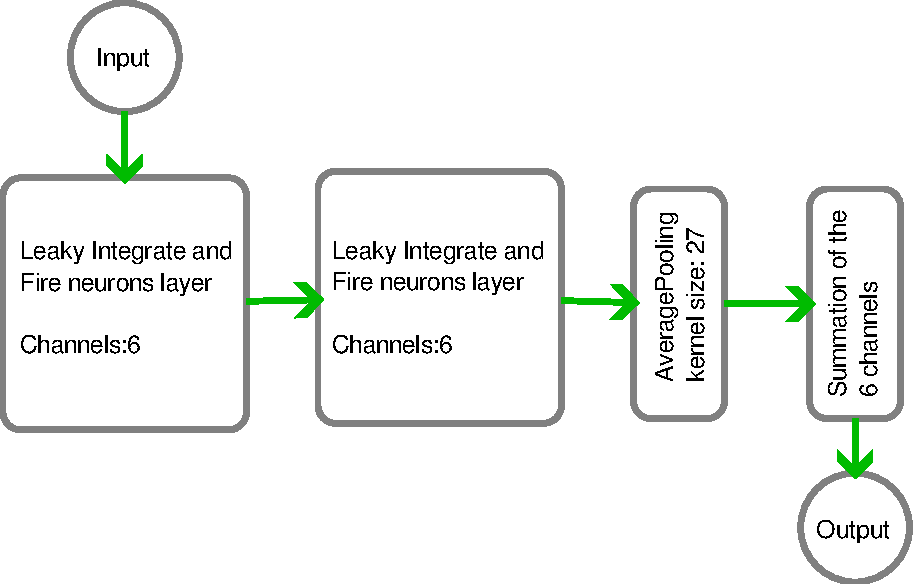
\includegraphics[width=.9\linewidth]{images/architectureSNN}
			\caption{Spiking neural network architecture}
			\label{fig:architecturesnn}
		\end{figure}
	
			\input{listings/snnArchitecture.py}
	
	
		\subsection{Convolutional layer with full connected sigmoid neurons CNN}
	
		\begin{figure}[H]
			\centering
			
\includegraphics[width=\linewidth]{images/architectureCNN}
			\caption{Convolutional neural network architecture}
			\label{fig:architecturecnn}
		\end{figure}
	
			\par The CNN were trained according to the following parameters:
			\begin{itemize}
				\item \textbf{random seed}: 42
				\item \textbf{learning rate}: $2.10^{-4}$
				\item \textbf{test batch size}: 40\%
				\item \textbf{training batch size}: 60\%
				\item \textbf{number of epochs}: 3000
				\item \textbf{loss function}: Cross-entropy
				\item \textbf{optimizer}: Adam ($0.00001 \leq \beta \leq 0.999$)
			\end{itemize}
			\input{listings/cnnArchitecture.py}
			\onecolumn
			
		\subsection{Results}
			\subsubsection{Results for CNN}
				\par The CNN exhibit some unstable behavior and had a poor convergence as seen in Figure \ref{fig:cnnacculoss}. Its stats are the following:
				\begin{itemize}
					\item Maximum Accuracy: 4.82\%
					\item Minimum Loss: 0.9468
					\item Average Accuracy: 1.23\%
					\item Average Loss: 3.328
				\end{itemize}
				
				\begin{figure}[H]
					\centering
					
\includegraphics[width=\linewidth]{images/cnnAccuLoss}
					\caption{CNN stats over 3000 epochs}
					\label{fig:cnnacculoss}
				\end{figure}
		
			\subsubsection{Results for SNN}
				\par The SNN exhibit a more stable behavior and had a better convergence then CNN as can be seen in Figure \ref{fig:snnacculoss}. Its stats are the following:
				\begin{itemize}
					\item Maximum Accuracy: 100.00\%
					\item Minimum Loss: 0.9278
					\item Average Accuracy: 18.25\%
					\item Average Loss: 3.296
				\end{itemize}
				\begin{figure}[H]
					\centering
					
\includegraphics[width=\linewidth]{images/snnAccuLoss}
					\caption{SNN stats over 3000 epochs}
					\label{fig:snnacculoss}
				\end{figure}
			

		
			\twocolumn
	
	
	
